
%% bare_conf.tex
%% V1.4b
%% 2015/08/26
%% by Michael Shell
%% See:
%% http://www.michaelshell.org/
%% for current contact information.
%%
%% This is a skeleton file demonstrating the use of IEEEtran.cls
%% (requires IEEEtran.cls version 1.8b or later) with an IEEE
%% conference paper.
%%
%% Support sites:
%% http://www.michaelshell.org/tex/ieeetran/
%% http://www.ctan.org/pkg/ieeetran
%% and
%% http://www.ieee.org/

%%*************************************************************************
%% Legal Notice:
%% This code is offered as-is without any warranty either expressed or
%% implied; without even the implied warranty of MERCHANTABILITY or
%% FITNESS FOR A PARTICULAR PURPOSE! 
%% User assumes all risk.
%% In no event shall the IEEE or any contributor to this code be liable for
%% any damages or losses, including, but not limited to, incidental,
%% consequential, or any other damages, resulting from the use or misuse
%% of any information contained here.
%%
%% All comments are the opinions of their respective authors and are not
%% necessarily endorsed by the IEEE.
%%
%% This work is distributed under the LaTeX Project Public License (LPPL)
%% ( http://www.latex-project.org/ ) version 1.3, and may be freely used,
%% distributed and modified. A copy of the LPPL, version 1.3, is included
%% in the base LaTeX documentation of all distributions of LaTeX released
%% 2003/12/01 or later.
%% Retain all contribution notices and credits.
%% ** Modified files should be clearly indicated as such, including  **
%% ** renaming them and changing author support contact information. **
%%*************************************************************************


\documentclass[conference]{IEEEtran}
\usepackage{cite}
\usepackage[pdftex]{graphicx}
 % \graphicspath{{../pdf/}{../jpeg/}}
 % \DeclareGraphicsExtensions{.pdf,.jpeg,.png}
\usepackage{amsmath}
%\usepackage{algorithmic}
%\usepackage{array}
%\usepackage{url}
% correct bad hyphenation here
\hyphenation{op-tical net-works semi-conduc-tor}


\begin{document}
\title{Report 2\\Related Work and Design}

\author{\IEEEauthorblockN{Filippo Bernardi}
\IEEEauthorblockA{Bologna University, Italy\\
Tongji University, China\\
TU/e, Netherlands\\
Email: filippobernardi@outlook.it}
\and
\IEEEauthorblockN{Snorri Stefánsson}
\IEEEauthorblockA{University of Reykjavik, Iceland\\
TU/e, Netherlands\\
Email: snorriste@gmail.com}
\and
\IEEEauthorblockN{Jonas Wallmeier}
\IEEEauthorblockA{Technical University Ilmenau, Germany\\
TU/e, Netherlands\\
Email: j.a.wallmeier@student.tue.nl}}

% make the title area
\maketitle

\begin{abstract}
Description of a wireless application for monitoring vital signs of plants and for supporting the user to maintain them alive. \\

\end{abstract}

% For peerreview papers, this IEEEtran command inserts a page break and
% creates the second title. It will be ignored for other modes.
\IEEEpeerreviewmaketitle
\hfill \today
\\

%Application description and exact scenario including research and/or industrial motivation

%Literature survey on similar applications (research or industry) and their solutions


%Intended protocol stack and justification for tha

%Network architecture options

%The method and tools for implementation (simulation, hardware platform, ...)

%Hardware/software implementation plan

%I but this here to prevent the pagebreaks inbetween the include{file} :) happy happy hippo filippo
\begingroup
\let\clearpage\relax
%(Application description and exact scenario including research and/or industrial motivation)
\section{Application description}
Keeping plants alive can be a very time consuming task: it requires knowledge about different types of plants as well as periodical checks if these requirements are fulfilled. 
The main idea behind this application is to create a network of nodes, placed directly in the soil of each plant, that, connected to a main hub, helps the user to keep all the plants healthy. Moreover, each node has a series of sensor to measure some of the environmental indexes, e.g. temperature or humidity. The Main-Hub device receives all the sensors data from each node and stores it in a database. This hub uses the contributed data from each plants and checks if it's acceptable for the type of plant the user defined. Via an user friendly web interface, the costumer can then easily view all information provided by the Hub.\\
The application is suitable for many type of buildings but in this paper it will be assumed to be operating in a large family house with a garden of reasonable size. The plant monitoring system should work indoor and outdoor. Even though plants might not be exposed to rain, all nodes should be waterproof since they are placed directly on the soil of the plant. However, in this project the robust final design will not be implemented in relations to water resistance and more focus is put on protocols and application layer.\\
Each node has numerous sensors which will inform the user of necessary actions needed to be taken. In this paper we describe only the sensors available on Texas Instrument's SensorTag CC2650. In further development additional sensors can we added to the node.
 \\

%Literature survey on similar applications (research or industry) and their solutions
\section{similar applications}
There are many plant monitoring system already available on the market. However, most of them use a smart phone as a host without creating a sensor network. It is important to bare in mind that the companies do not declare which protocols are used and therefore information is limited. Nevertheless, some assumptions could be reliably made from the data provided. The following devices demonstrate an overview of existing solutions:\\
\begin{enumerate}
	\item Edyn \cite{Edyn} \\
This application is called Edyn, is composed by a device that has to be placed in the soil. Moreover, is has sensors for light, moisture, humidity and is able to inform its users about the nutrition status of the plant. There is a solar panel integrated on top of the device to power the device and charge its battery. The apparatus connects to a WiFi network and communicates with a smart phone via app where all the information is shown. The system uses a actuator, a automatic watering system, enabled upon information from its partner device.\\
\item PlantLink \cite{MyPlantlink}\\
PlantLink is a system which can sense the moisture of a plant and wirelessly communicate with a base station. This base station can be paired with up to 64 sensors nodes. There is a smartphone app that informs the users about the health levels of the plant. Each sensor is associated to a specific type of plant by the user and the system can then look up generic requirements for that plant and advice the user accordingly. The system also has a PlantLink valve, a specific actuator able to water the system automatically. The user can also control the actuator through the app if required. This application seems to be different from the amount of sensors in the system. Therefore, PlantLink is restricted to the humidity of the plant whereas the other solutions mentioned here provide multiple sensor values and meet more requirements of the users.\\

\item Parrot Flower Power \cite{parrot}\\
This third application available on the market is composed of a device that has to be placed directly on the soil of plant to monitoring, like the others. It does not have any actuator and reports to the user via smart phone app. The system is battery powered that can be easily changed and it also come with integrated light, moisture and temperature sensors. This device communicates straight to a smart phone via bluetooth.
\end{enumerate}

\subsection{Conclusion of existing devices}

The described solutions listed show the general purpose and requirements of a plant monitoring systems. User requirements are the most important aspect of each of these systems and have to be taken into account in the design. By looking at the those three systems, they all report the valuable information to the user in a comfortable way but some of them lack the off site connectivity and scalability of the amount of sensor nodes and range, which is vital for some plants in order for them to stay alive. 

 
%Detailed hardware setup (processor, RF, sensors, battery, memory, etc.)
\section{Detailed hardware setup}

The wireless network system consists of a Hub and sensor nodes. After careful examination of all available nodes the Multi-standard SensorTag from Texas instruments \cite{TIsensortag} was chosen. A Crossbow Telos B node has been used as sink for the network and as interface with the Raspberry Pi board. 
Initially, a completely different system was designed. It was made with an XigBee board as a link between the nodes and the Raspberry pi. However, because of lack of documentation of the SensorTags and its actual zigbee protocol support, development with it could not continue. Instead, the highly research and documented TelosB Crowbow node was preferred.


\subsection{Sensor Node - TI Sensor Tag}

The General requirements for the node were design for durability, optimal functionality and user friendly application. This sensor application requires many precise design parameters from the node but those can not all be satisfied. Thus, the general requirements will be discussed and then shown how well the TI sensor tag fulfills them and how it could be added. With the time scope of the project, some of these requirements will not be met, rather a focus will be but on functionality of current components.

In general the nodes have to be small in size to fit even in small plant pots. They should be battery powered and in order to be able to acquire the necessary data, they need to have sensors in and above the soil. Moreover, the nodes should be waterproof, contain a status-LED and a RF-module for wireless communication with the Hub.

Each sensor node should be able to measure the items listed in Table \ref{list-req} and if the sensor tag fulfills them or not.
\begin{table}[htbp]
	\centering
	\begin{tabular}{lc}
		\toprule
		Requirements & \multicolumn{1}{l}{TI sensor tag} \\ 
		\midrule
		Brightness & yes \\ 
		Temperature & yes \\ 
		Soil humidity & no \\ 
		Air humidity & yes \\ 
		Soil Ph-value & no \\
		\bottomrule 
	\end{tabular}
	\vspace{0.1cm}
	\caption{Requirement compared to the capabilities of the TI sensor tag}
	\label{list-req}
\end{table}


A high sampling rate is not necessary and therefore keeping the sampling rate to a minimum increases battery life substantially. For the same reason it is advisable to decrease the transmission rate by only sending data upon significant change.

\subsubsection{Detailed hardware design}

The sensor tag from TI can measure many things which are useful for the project and was chosen were it also offers various connection methods via BLE, Zigbee, 6LowWPAN and soon wifi. Its battery lasts a year with one second report intervals and is easily replaceable be the user. 

The multi-standard processor, CC2560 \cite{block-cc2650}, connects to ten low power MEMS (Microelectromechanical systems) \cite{MEMS} sensors seen in Figure \ref{fig:sensors}. This makes it possible to be extremely small (micrometers), light weight, mobile and robust.

\begin{figure}[!h]
	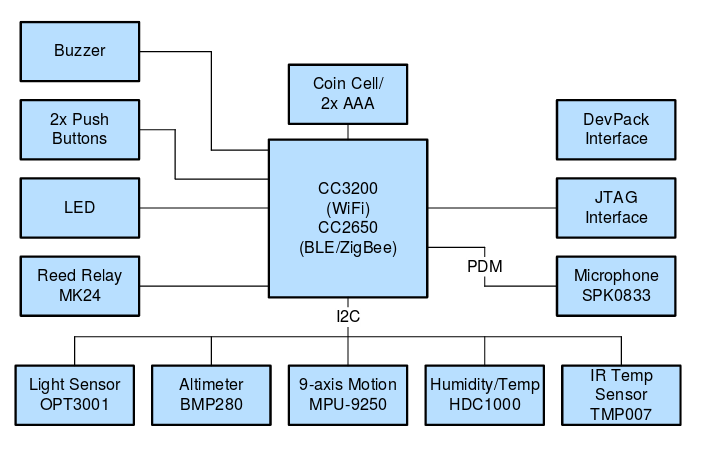
\includegraphics[width=\linewidth]{sensors-layout}
	\caption{Block diagram of the MEMSs sensors and the CC2650 processor \cite{block-cc2650}.}
	\label{fig:sensors}
\end{figure}


\subsection{Hub - Raspberry Pi 3}
The Hub has to be able to collect all data provided from the nodes. It can be connected to the buildings power grid and Internet. A user interface (UI) should be digitally accessible via touchscreen, web page and/or app. Additionally the system should be able to inform the user about critical sensor values. To decide whether a value is critical or not, the Hub has to know which type of plant the sensor monitors and then check a Internet database for specific requirements or rely on user defined values.
The Raspberry pi 3, will be referred to as the Pi, is able to connect to the internet via wifi or ethernet without extra adapters. The Pi used in this application is 3 model b that differ from the previous hardware because the addition of A
802.11n Wireless LAN, the Bluetooth 4.1 and Bluethooth Low Energy (BLE). Furthermore, the processos has been upgraded to a 1.2GHz 64-bit quad-core ARMv8 CPU. \cite{pi}\\

\subsection{Crossbow TelosB}
In this application also another type of node has been used: Crossbow TelosB. It is developed by the University of California, Berkley and it is based on the open source TelosB / Tmote Sky platform. 
The main advantages of this sensor node is the presence of a USB hardware interface for direct communication with the Pi. The node will used as a link between the Raspberry and the sensor network composed of the TI sensortag nodes, see Figure \ref{fig:Architecture}.
The Crossbow TelosB is equipped with a 802.15.4 compliant transceiver, humidity, temperature and light sensor and it is powered by 2 AA batteries. The node is able to run Contiki and TinyOs \cite{TB}.\\



\section{Protocol stack}
\subsection{Overview}
The main objective is to create an interface between the wireless sensor network via IEEE 802.15.4 and the internet. This interface, made by the Raspberry pi, is needed because the data that has to be sensed by the wireless sensor network, has to be available on a web page, letting the user analyze them. \\
\subsection{IEEE 802.15.4}
IEEE 802.15.4 is standardized for Low-power wireless Personal Area Networks (LP-WPANs). It covers the physical and medium access control layers and there have been released three versions since 2003.
In IEEE 802.15.4 the Physical layer operates in 27 channels: 1 in 868MHz, 10 in 902MHz and 16 in 2.4GHz frequency. The data transfer rate is up to 250 Kbps.\cite{slide}\\
\subsection{Network Topologies}
In this section, the network architecture of a plant monitoring system will be discussed. \\
Firstly, the IEEE 802.15.4 regulation defines two types of node: the Full Function Device (FFD) and Reduced Function Device (RFD). The RFD differs from the other were it has reduced functional capabilities: it can not forward data from one node to another nor be a coordinator for other nodes of the network. Therefore, it is a device with fewer resources that can only send messages to other nodes. The final network is composed by a main FFD referred to as a Pan coordinator, the Full Function Devices as the co-coordinator and all the other RFD as End device. \cite{802154} \\
Secondly, the standard defines some topology configuration of the network. The most simple one is the star topology. It is composed by a central pan coordinator that is connected with all other devices. Each device sends data to the pan coordinator and no need to have a node that forwards messages. Moreover, in this type of architecture there are not any node dependence to let data arrive to the main hub.\\
Another type is the tree topology. This has the peculiarity of having a family group of node that send data to a central co-coordinator node which in turn froward the messages to the Pan coordinator. The advantage of this topology it the increased range of communication that the overall network is able to exploit.
Finally, the peer-to-peer communication is an ad hoc network where most of the nodes are FFD. Therefore, each node has not only a central co-coordinator but they are also interconnected with each other creating a network of routed communication. This system is more reliable from the previous one were, in the case of a failure of a co-coordinator node, no other nodes are lost compared to tree topology were all child nodes would be lost. In peer-to-peer, the network is able to adapt and fix this failure using the other communication channels.\\
The hardware used in the application discussed in this paper is: a Raspberry Pi board with a TelosB board for communication will be the pan coordinator and SensorTag by Texas Instrument for all the other node. The choice of a proper network architecture for a plant monitoring system is particularly related to the place of application of this system. Furthermore, in case the system is located in a small house the star topology will be a satisfactory choice. In case of more spacious area where the range between two node is longer, a peer-to-peer topology will be preferred. In case of a multiple leveled building, a pan coordinator on each floor would be required.\\
Nevertheless, because this application uses 6lowPan protocol (will be discussed later on this paper) a mesh topology, previously discussed with peer-to-peer name, will be used.
\\



\subsection{MAC Requirements}
For choosing the suitable MAC-Layer for the system, the following requirements have to be considered:

\begin{itemize}
	\item \textbf{Datarate:}
	Low. All that has to be transmitted by the plants are some sensor values. Therefore a low datarate is sufficient.
	\item \textbf{Network Size:}
	Big. All Nodes have to be connected to the Hub. In order for the system to be able to operate in small apartments as well as in large buildings, it should provide multihop capabilities.
	\item \textbf{Energy Consumption:}
	Very Low. The system consists of several battery powered nodes that can be spread over a large area. Therefore, changing batteries can be very time consuming and should be made as avoidable as possible.
	\item \textbf{Latency:}
	Uncritical. The monitored values are usually changing relatively slow so that real-time measuring is not necessary.
\end{itemize}

While CSMA-Approaches are usually a good choice for low-traffic, multi-hop networks always require some kind of synchronization for making it energy efficient, which is not provided by CSMA.\\
TDMA-Approaches on the other hand are easily applied in multi-hop networks. However, TDMA is relatively inflexible to a changing network topology and generally a bad choice for low-traffic networks.\\
In IEEE 802.15.4 CSMA/CA is used. The protocol works as follows:
the sender wait until the channel is idle, if it is the case, the sender wait for a random back-off period and then it send the data. The receiver, if the data are correctly received, send back an acknowledgment packet back to the sender. Naturally, if the sender do not sense the acknowledgment packet, it start to send again the data.\\

\subsection{un-slotted CSMA}
IEEE 802.15.4 can use slotted or un-slotted CSMA procedure. Here the un-slotted procedure will solely be discussed because it is implemented in the plant monitoring system. The un-slotted procedure is as follow: after an initialization phase, the system waits for a random back-off period. Thereafter it uses clear channel assessment (CCA), it checks if the channel is idle or not. If the channel is idle the procedure succeeds otherwise the node backs off. The system repeats from the backoff period until the channel is idle or the backoff procedure has reached the maximum allowed times. This cause a failure in the procedure.\\


\subsection{6LowPAN}
6LowPAN stands for IPv6 over Low Power Wireless Personal Area Networks and it is based on the IEEE 802.15.4 protocol. Ipv6 is a relatively new type of Internet protocol and it has been made for handle the increasing amount of devices that are connected to the Internet. It differs from the IPv4 were it uses a much longer IP \cite{6lowpan}.\\
6LowPAN standards has been developed for connecting embedded devices on the Internet via IPv6.\cite{why}
The main advantage of having an IP in a IEEE 802.15.4 device is that a node is able to use directly an IP network without the use of any other interface. Moreover, a node with an IP address is able to use an pre-built infrastructure. These features meet some general requirements of IoT, Internet of Things: smart devices that collect data and upload them directly to the Internet.
However, there is one main issues in 6loWPAN: the difference packet size between the IEEE 802.15.4 and the IPv6. Firsly, in IEEE 802.15.4 the payload is 102 bytes but actual packet is 127 bytes in total, in these 127 bytes there are 25 bytes of frame overhead that are not part of the data. On the other hand, in IPv6 the packet length is of 1280 bytes. This means that it is necessary to do a fragmentation and a reassembly of the packet for converting the IPv6 packet to an IEEE 802.15.4 format. Moreover, a compression of header field is necessary.\\
To conclude, the 6LowPAN is based on IEEE 802.15.4 standard where a un-slotted CSMA/CA is used. The node architecture used is the mesh type. These two characteristics are a good match, even if there are some constrains between those standards, especially for the plant monitoring system.

\section{Network architecture}
Using all the concept described in the previous sections it is possible to describe the plant monitoring system application. All the following steps has been made by using the guide developed by Laurent Deru, Sébastien Dawans and Mathieu Ocana, available in GitHub under permissive 3-clause BSD-style open source license. However, in the tutorial it is used only TelosB node instead of the Texas Instrument Sensor Tags that is used in this development of a plant monitoring system.\\
\begin{figure}[!h]
	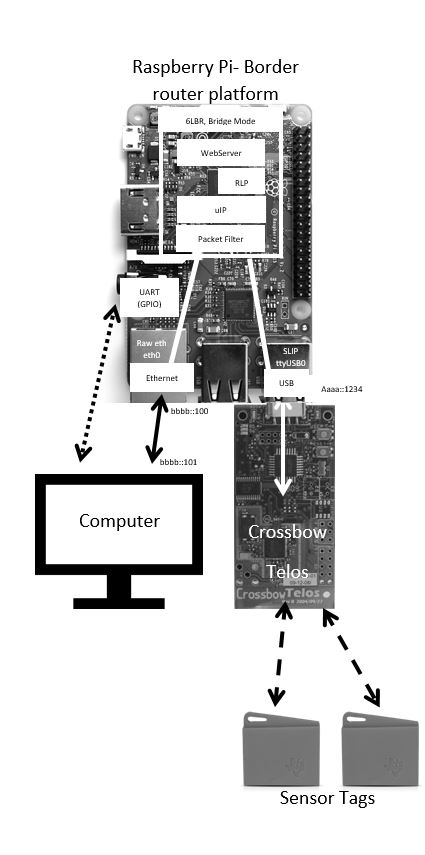
\includegraphics[width=\linewidth]{Network}
	\caption{Development of the network}
	\label{fig:Network}
\end{figure}
\subsection{The network}
The network main idea is well depicted in fig\ref{fig:Network}. The raspberry pi act as a six low pan border router (6LBR) and act as a link between the Ethernet and the wireless sensor network. The wireless sensor network is composed by the TelosB that act as a sink for all the other sensor tags. The TelosB sensor is attached via USB to the Raspberry Pi.
On the other hand, the Raspberry Pi is connected to a computer via a normal house router.\cite{6LBR}
The Raspberry Pi connect the two subnets via RPL protocol on the wireless sensor network side and NPD on the Ethernet part.\cite{mode}\\
\subsection{WebServer}





\section{Development}

Each component of the project had to be developed individually before assembling them together into a working prototype. The Raspberry Pi, the router, the Sensor Tag and the TelosB. A description of each devices configuration will be described and then how the connection is made between each of them.\\

A good overview of the project can be seen in Figure \ref{fig:over}.

\begin{figure}[!h]
	\begin{center}
		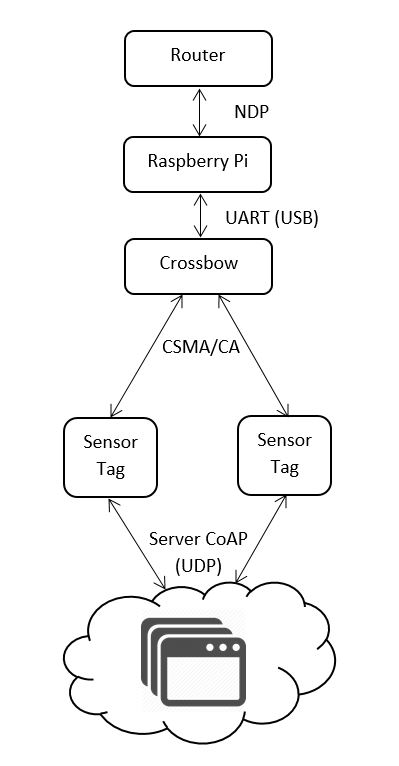
\includegraphics[width=0.6\linewidth]{protocol}
		\caption{sensor node connected with the debugger to a computer}
		\label{fig:over}
	\end{center}
\end{figure} 

\subsection{Raspberry pi - 6LoWPAN Boarder Router}

The Raspberry Pi acts as a boarder router for the WSN in Smart brigde mode. It mitigates information to from the WSN mesh into the IPv6 network of the router. The boarder router is installed into the Raspberry pi via the 6LBR-1.3.3 Packages for Raspian. The service can be started through the terminal and the status of the working service can be seen in Figure \ref{fig:router}.

\begin{lstlisting}[basicstyle=\small,language=bash,caption={Start the 6lbr service and check the status}]

$ sudo 6lbr service start
$ sudo service 6lbr status
  6lbr.service - LSB: 6LoWPAN Border Router
Loaded: loaded (/etc/init.d/6lbr)
Active: active (running); 1h 32min ago
\end{lstlisting}

After making sure that the bridge boarder router is configured correctly (see the documentation on the 6lbr github page for configuring a rapsberry pi connection), the TelosB should be connected the the Raspberry Pi and the IPv6 address can be found be running: 
 
\begin{lstlisting}[basicstyle=\small,language=bash,caption={Get the TelosB node IPv6 address for accessing the 6lbr client}]

$ cat /var/log/6lbr.ip 
2002:aaa:2e10:10:212:7400:13ea:961
\end{lstlisting}

This address can then be used to access the 6lbr client directly as seen in Figure \ref{fig:interface}.

\begin{figure}[!h]
	\begin{center}
		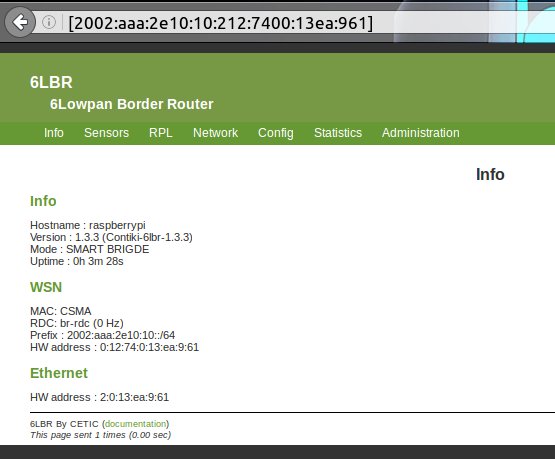
\includegraphics[width=1\linewidth]{interface}
		\caption{The 6lbr interface on the pi}
		\label{fig:interface}
	\end{center}
\end{figure} 

\subsection{Router}

The router has to be configured to IPv6 network as well to be able to communicate with the 6LoWPAN network and assign IPv6 addresses to devices that want to access the nodes via CoAP, even mobile phones. The router was configured to 6to4 (converting IPv6 to IPv4 traffic), see Figure \ref{fig:routerSettings} with RADVD.

\begin{figure}[!h]
	\centering
		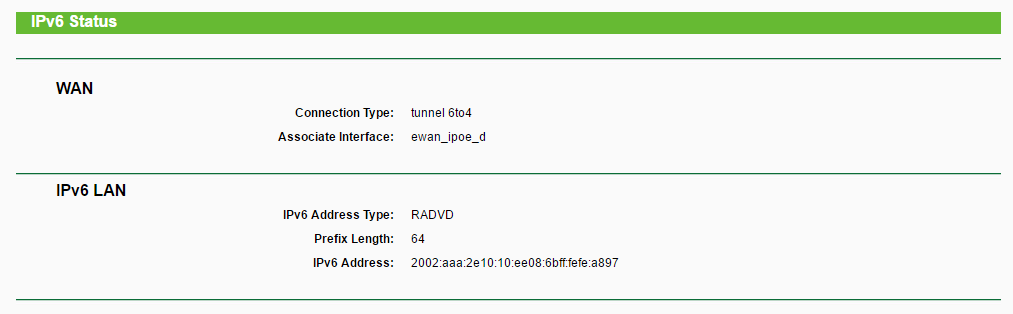
\includegraphics[width=1\linewidth]{routerSettings}
		\caption{The router settings needed for communicating within the LAN to the WSN}
		\label{fig:routerSettings}
\end{figure} 

\subsection{TI Sensor Tag - Sensor nodes}

The sensor tag communicates to the TelosB via 802.15.4. For working with the tag, a special software (Windows only) has to be used to upload a binary file to it see the next Section \ref{sec:flash}. First the code that is supposed to be used has to be cross compiled on a Linux machine. For the communication with the TelosB, the contiki library was used for the sensor tags processor family, more specific: "/contiki/examples/cc26xx/cc26xx-web-demo/cc26xx-web-demo.c". In order to compile it the following command should be run:

\begin{lstlisting}[basicstyle=\small,language=bash,caption={Cross compiling the web-demo to a binary file for the sensor tag}]

cd contiki/examples/cc26xx/cc26xx-web-demo/
nano project-conf.h
make TARGET=srf06-cc26xx BOARD=sensortag/cc2650
     cc26xx-web-demo.bin CPU_FAMILY=cc26xx
\end{lstlisting}

\begin{lstlisting}[basicstyle=\small,language=c,caption={The configurisation file for the web-demo in directory: contiki/examples/cc26xx/cc26xx-web-demo/project-confg.h}]

#define RF_BLE_CONF_ENABLED                 0
#define CC26XX_WEB_DEMO_CONF_MQTT_CLIENT    0
#define CC26XX_WEB_DEMO_CONF_6LBR_CLIENT    0
#define CC26XX_WEB_DEMO_CONF_COAP_SERVER    1
#define CC26XX_WEB_DEMO_CONF_NET_UART       0
\end{lstlisting}

These commands create a binary file "cc26xx-web-demo.bin" which can be flashed onto the sensor tag via the SmartRF Flash Programmer 2.


\subsubsection{Flashing the Texas Instrument Sensor-Tag} 
\label{sec:flash}
In order to flash the sensor tag, SmartRF Flash Programmer 2 made by Texas Instrument has been used. For flashing the node a sensor tag needs a Debugger DevPack, the debugger allows for communication to the sensor via USB as it is shown in Figure \ref{fig:debug}.  
\begin{figure}[!h]
	\begin{center} 	
		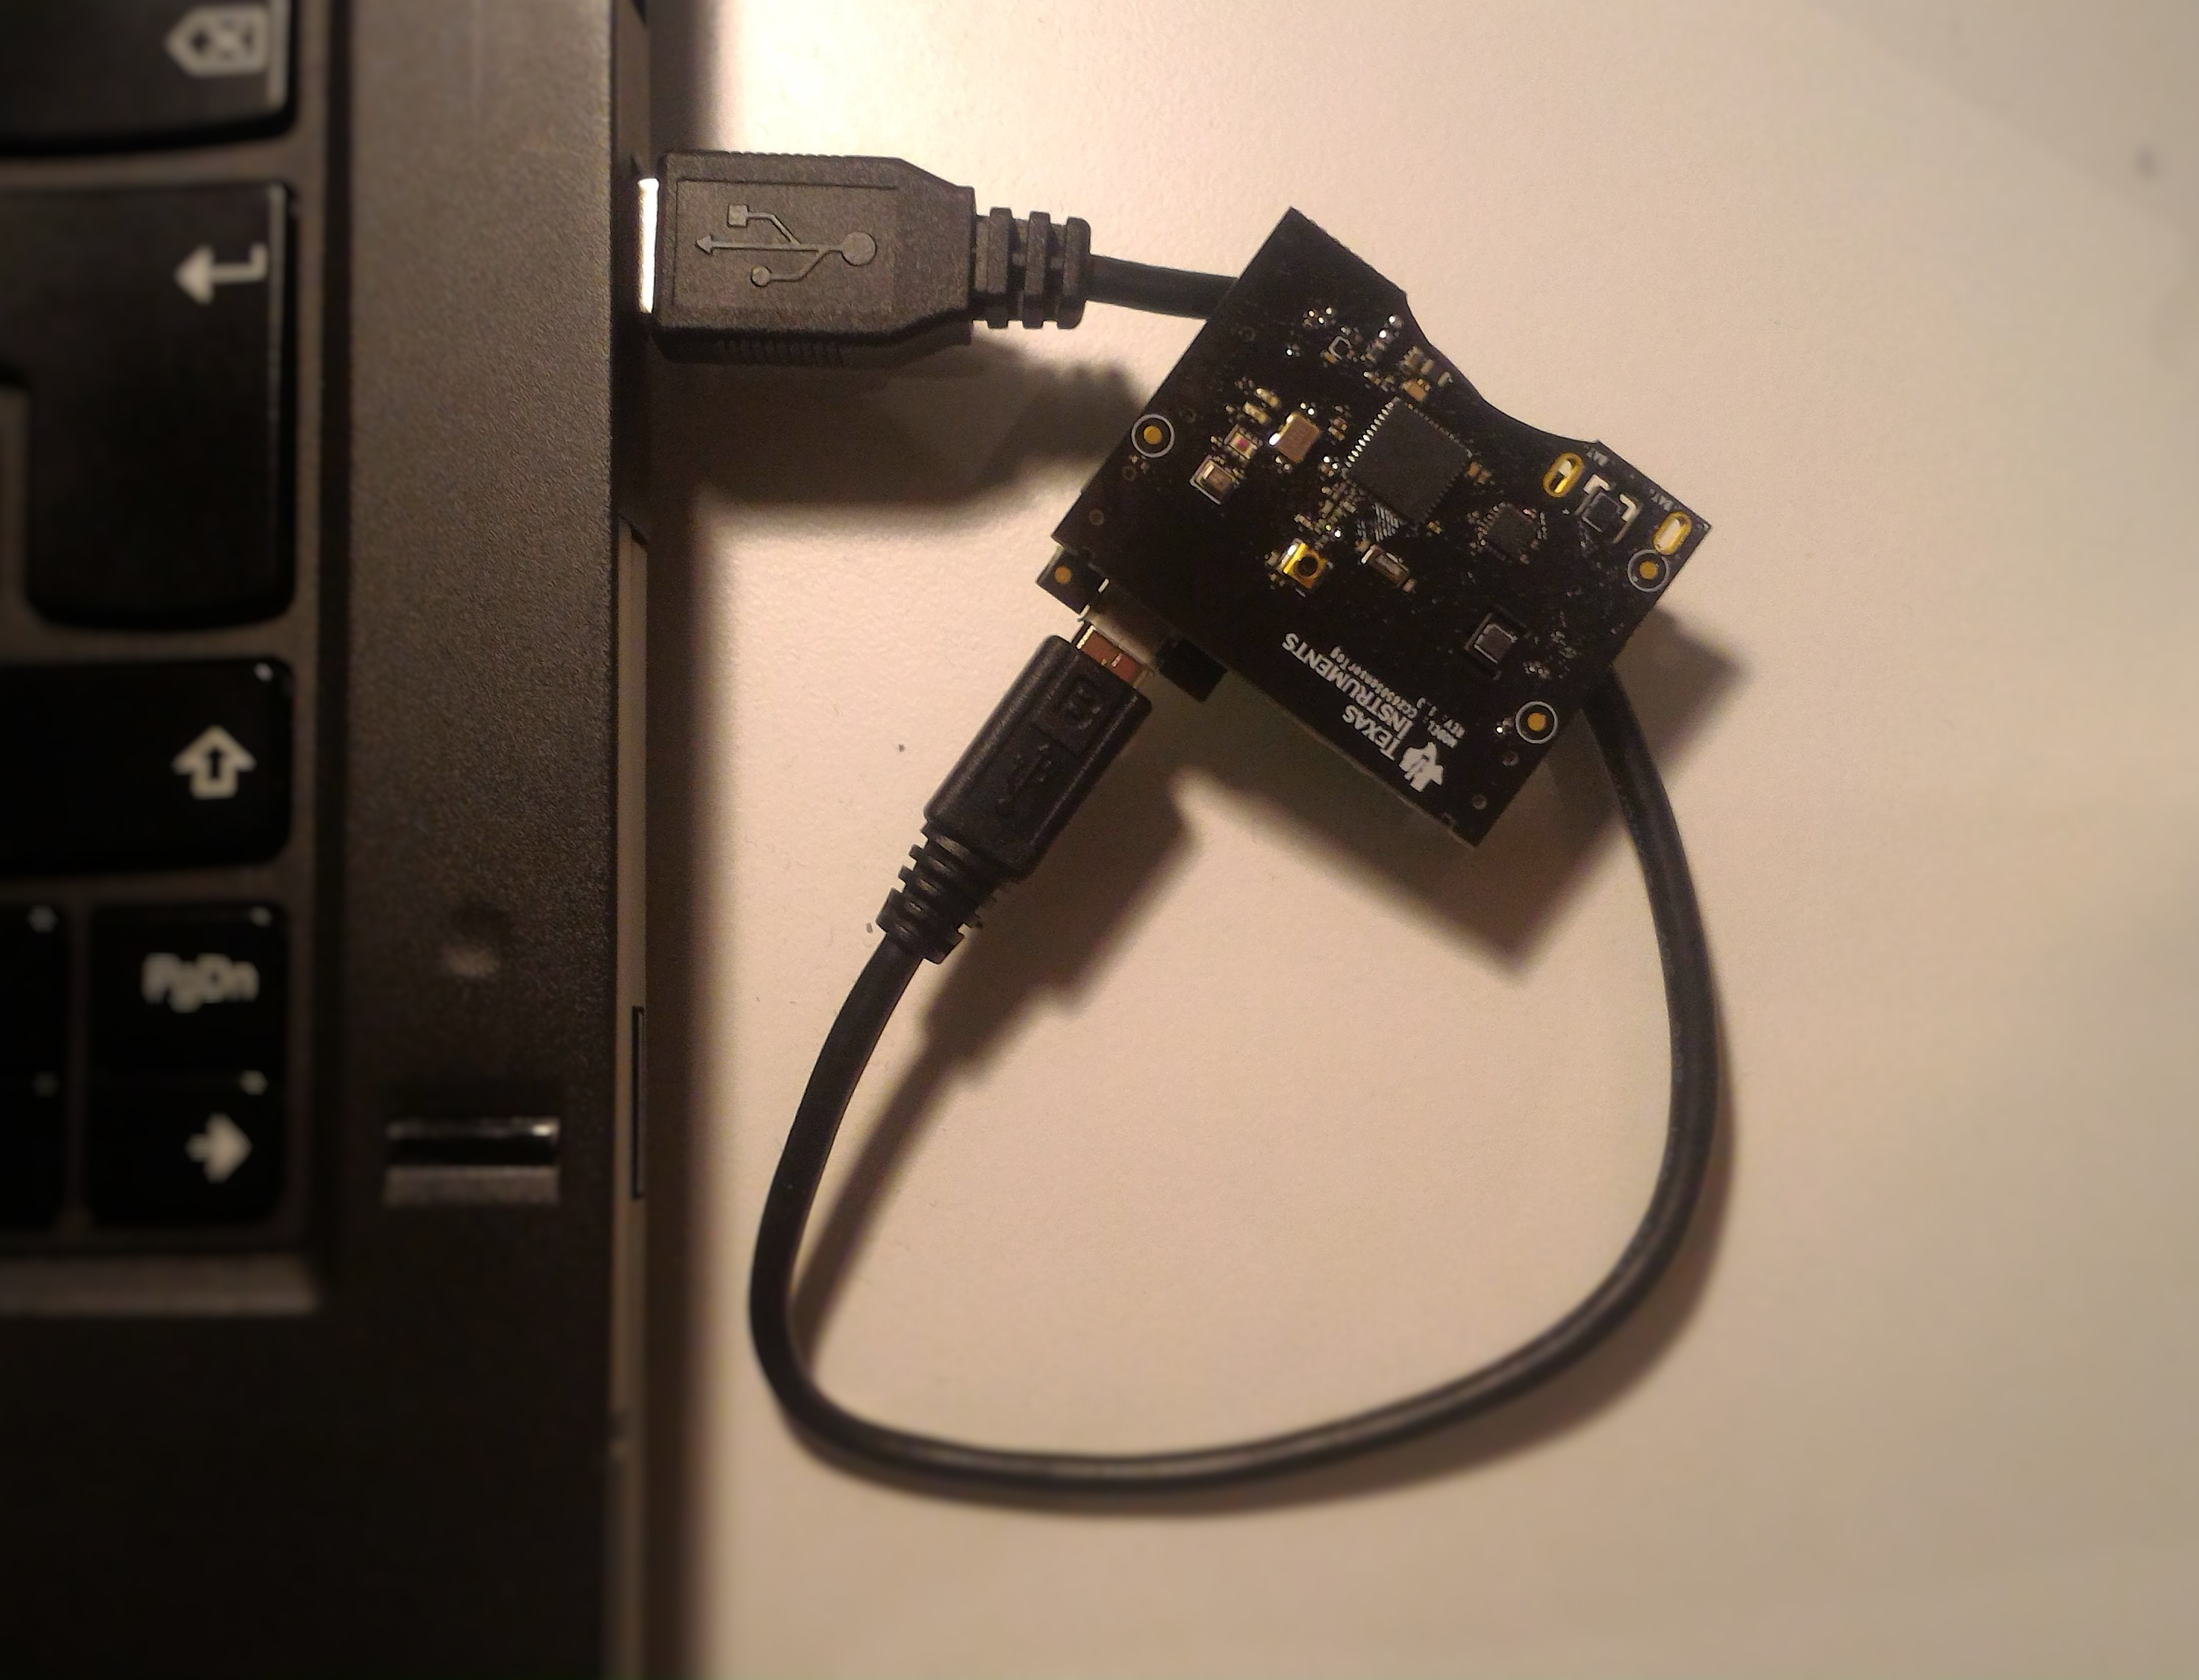
\includegraphics[width=0.8\linewidth]{debugger}
		\caption{sensor node connected with the debugger to a computer}
		\label{fig:debug}
	\end{center}
\end{figure} 

\subsection{Crossbow TelosB mote - slip-radio}
This allows the Pi to act as a network coordinator for the sensor tags in the 6loWPAN network via the 802.15.4 enabled transceiver on the Crossbow. The software on the Crossbow is a slip-radio, specially made for it by Contiki. The slip radio from Contiki has to be cross compiled and uploaded to the TelosB. First make sure the correct configuration is correct and then make/compile the code into a binary file and upload it to the mote.

\begin{lstlisting}[basicstyle=\small,language=bash,caption={Setting for the TelosB mote}]

#For TelosB Sky-Mote
cd contiki/examples/ipv6/slip-radio
#connect the device
#Configure the project-conf.h
nano project-conf.h
make TARGET=sky slip-radio.upload
\end{lstlisting}

\begin{lstlisting}[basicstyle=\small,language=c,caption={Setting for the TelosB mote}]

#define NETSTACK_CONF_MAC     nullmac_driver
#define NETSTACK_CONF_RDC  contikimac_driver
#define NETSTACK_CONF_NETWORK slipnet_driver
#define NETSTACK_CONF_FRAMER  no_framer
\end{lstlisting}


\section{Hardware and software implementation plan}


\begin{ganttchart}[
	vgrid,
	hgrid
	]{1}{12}
	\gantttitle{Implementation plan - Hardware \& software}{12} \\
	\ganttbar{Task 1}{1}{4} \\
	\ganttbar{Task 2}{5}{6} \\
	\ganttmilestone{M 1}{6} \\
	\ganttbar{Task 3}{7}{11}
	\ganttlink{elem0}{elem1}
	\ganttlink{elem1}{elem2}
	\ganttlink{elem2}{elem3}
\end{ganttchart}
\endgroup

\section{Design}
\subsection{Sensor Node}
The nodes have to be small in size to fit even in small plant pots. They should be battery powered and in order to be able to acquire the necessary data, they need to have sensors in and above the soil. Moreover, the nodes should be waterproof, contain a status-LED and a RF-module for wireless communication with the Hub.

Each sensor node should be able to measure the following:
\begin{itemize}
	\item Brightness
	\item Temperature
	\item Soil humidity
	\item Air humidity
	\item Ph-Value
\end{itemize}

However, a high sampling rate is not necessary and therefore keeping the sampling rate to a minimum increases battery life substantially. For the same reason it is advisable to decrease the transmission rate by only sending data upon significant change.

\subsection{Hub}
The Hub has to be able to collect all data provided from the nodes. It can be connected to the buildings power grid and Internet. A user interface (UI) should be digitally accessible via touchscreen, web page and/or app. Additionally the system should be able to inform the user about critical sensor values. To decide whether a value is critical or not, the Hub has to either know which type of plant the sensor monitors and then check a Internet database for specific requirements or rely on user defined values.


%\begin{figure}[!t]
%\centering
%\includegraphics[width=2.5in]{myfigure}
% where an .eps filename suffix will be assumed under latex, 
% and a .pdf suffix will be assumed for pdflatex; or what has been declared
% via \DeclareGraphicsExtensions.
%\caption{Simulation results for the network.}
%\label{fig_sim}
%\end{figure}

%\begin{figure*}[!t]
%\centering
%\subfloat[Case I]{\includegraphics[width=2.5in]{box}%
%\label{fig_first_case}}
%\hfil
%\subfloat[Case II]{\includegraphics[width=2.5in]{box}%
%\label{fig_second_case}}
%\caption{Simulation results for the network.}
%\label{fig_sim}
%\end{figure*}

%\begin{table}[!t]
%% increase table row spacing, adjust to taste
%\renewcommand{\arraystretch}{1.3}
% if using array.sty, it might be a good idea to tweak the value of
% \extrarowheight as needed to properly center the text within the cells
%\caption{An Example of a Table}
%\label{table_example}
%\centering
%% Some packages, such as MDW tools, offer better commands for making tables
%% than the plain LaTeX2e tabular which is used here.
%\begin{tabular}{|c||c|}
%\hline
%One & Two\\
%\hline
%Three & Four\\
%\hline
%\end{tabular}
%\end{table}
\begin{flushleft}
	
\section{Conclusion}
	The authors hope that this system will help people maintain their apartment green.
	The device described in this paper will be develop in  next two month creating a real prototype.
\end{flushleft}

\section{Bibliography}
\begin{itemize}
	\item https://www.edyn.com/
	\item https://myplantlink.com/how-it-works
	\item http://global.parrot.com/au/products/flower-power/
	
\end{itemize}



% that's all folks
\end{document}


